% 34-20(34쪽) — $y=2^{x}$, $y=8^{x}$ 의 그래프와 직선 $x=k$, 네 점 $\pt{A}$·$\pt{B}$·$\pt{C}$·$\pt{D}$(원문 「오른쪽 그림」). 스캔 화질이 낮아 TikZ 로 다시 그림.
% 라벨은 원문 것만: 두 그래프 이름, $y$축의 $1$, $x$축의 $k$, 직선 이름 $x=k$, 네 점 이름, $\pt{O}$.
% $\seg{BD}=l\seg{AC}$ 의 $l$(답)이 읽히지 않게 길이·좌표값은 적지 않는다.
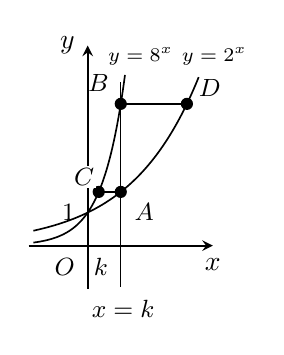
\begin{tikzpicture}[line width=0.6pt, x=0.60cm, y=0.42cm, >=stealth]
  \draw[->, line width=0.7pt] (-1.25,0) -- (2.65,0) node[below=1pt] {$x$};
  \draw[->, line width=0.7pt] (0,-1.30) -- (0,6.05) node[left=1pt] {$y$};
  \draw[line width=0.5pt] (0.7,-1.25) -- (0.7,4.95);
  \draw[domain=-1.15:2.35, samples=90, smooth] plot (\x, {pow(2,\x)});
  \draw[domain=-1.15:0.79, samples=90, smooth] plot (\x, {pow(8,\x)});
  \draw[line width=0.5pt] (0.2333,1.6245) -- (0.7,1.6245);
  \draw[line width=0.5pt] (0.7,4.2871) -- (2.1,4.2871);
  \fill (0.7,1.6245) circle (2.2pt);
  \fill (0.7,4.2871) circle (2.2pt);
  \fill (0.2333,1.6245) circle (2.2pt);
  \fill (2.1,4.2871) circle (2.2pt);
  \node[anchor=north west, font=\small] at (0.78,1.58) {$\pt{A}$};
  \node[anchor=south east, font=\small] at (0.66,4.36) {$\pt{B}$};
  \node[anchor=south east, font=\small, fill=white, inner sep=0.8pt] at (0.20,1.72) {$\pt{C}$};
  \node[anchor=south west, font=\small] at (2.14,4.22) {$\pt{D}$};
  \node[anchor=east, font=\small] at (-0.06,1.0) {$1$};
  \node[anchor=north east, font=\small] at (-0.06,-0.08) {$\pt{O}$};
  \node[anchor=north east, font=\small] at (0.64,-0.08) {$k$};
  \node[anchor=north, font=\small] at (0.75,-1.35) {$x=k$};
  \node[anchor=south west, font=\scriptsize] at (0.22,5.15) {$y=8^{x}$};
  \node[anchor=south west, font=\scriptsize] at (1.78,5.15) {$y=2^{x}$};
\end{tikzpicture}
